% \documentclass[10pt]{article} 

\usepackage{amsmath,amssymb,amsthm,amsfonts} % assumes amsmath package installed
\usepackage[linktocpage=true,colorlinks=true,linkcolor=blue,citecolor=blue,urlcolor=blue]{hyperref}
\usepackage[letterpaper,margin=0.9in]{geometry}

% \newtheorem{definition}{Definition}
% \newtheorem{assumption}{Assumption}
% \newtheorem{theorem}{Theorem}
% \newtheorem{conjecture}{Conjecture}
% \newtheorem{lemma}{Lemma}
% \newtheorem{proposition}{Proposition}
% \newtheorem{remark}{Remark}

\newcommand{\bx}{\boldsymbol{x}}
\newcommand{\be}{\boldsymbol{e}}
\newcommand{\blambda}{\boldsymbol{\lambda}}
\newcommand{\bLambda}{\boldsymbol{\Lambda}}
\newcommand{\bu}{\boldsymbol{u}}
\newcommand{\bw}{\boldsymbol{w}}
\newcommand{\by}{\boldsymbol{y}}
\newcommand{\bz}{\boldsymbol{z}}
\newcommand{\bV}{\boldsymbol{V}}
\newcommand{\bX}{\boldsymbol{X}}
\newcommand{\bY}{\boldsymbol{Y}}
\newcommand{\bZ}{\boldsymbol{Z}}
\newcommand{\bv}{\boldsymbol{v}}
\newcommand{\bxi}{\boldsymbol{\xi}}
\newcommand{\bpi}{\boldsymbol{\pi}}
\newcommand{\bphi}{\boldsymbol{\phi}}
\newcommand{\bbeta}{\boldsymbol{\eta}}
\newcommand{\bpsi}{\boldsymbol{\psi}}
\newcommand{\bzeta}{\boldsymbol{\zeta}}
\newcommand{\bmu}{\boldsymbol{\mu}}
\newcommand{\bq}{\boldsymbol{q}}
\newcommand{\bQ}{\boldsymbol{Q}}
\newcommand{\bK}{\boldsymbol{K}}
\newcommand{\bP}{\boldsymbol{P}}
\newcommand{\bS}{\boldsymbol{S}}
\newcommand{\bT}{\boldsymbol{T}}
\newcommand{\bF}{\boldsymbol{F}}
\newcommand{\bG}{\boldsymbol{G}}
\newcommand{\bd}{\boldsymbol{d}}
\newcommand{\bp}{\boldsymbol{p}}
\newcommand{\bff}{\boldsymbol{f}}
\newcommand{\bc}{\boldsymbol{c}}
\newcommand{\bg}{\boldsymbol{g}}
\newcommand{\bh}{\boldsymbol{h}}
\newcommand{\bA}{\boldsymbol{A}}
\newcommand{\bL}{\boldsymbol{L}}
\newcommand{\ba}{\boldsymbol{a}}
\newcommand{\bb}{\boldsymbol{b}}
\newcommand{\bB}{\boldsymbol{B}}
\newcommand{\bC}{\boldsymbol{C}}
\newcommand{\bE}{\boldsymbol{E}}
\newcommand{\bH}{\boldsymbol{H}}
\newcommand{\bR}{\boldsymbol{R}}
\newcommand{\bn}{\boldsymbol{n}}
\newcommand{\bm}{\boldsymbol{m}}
\newcommand{\br}{\boldsymbol{r}}
\newcommand{\bl}{\boldsymbol{l}}
\newcommand{\bI}{\boldsymbol{I}}
\newcommand{\osigma}{\overline{\sigma}}
\newcommand{\usigma}{\underline{\sigma}}
\newcommand{\oosigma}{\overline{\osigma}}
\newcommand{\uusigma}{\underline{\usigma}}
\newcommand{\olambda}{\overline{\lambda}}
\newcommand{\ulambda}{\underline{\lambda}}
\newcommand{\oolambda}{\overline{\olambda}}
\newcommand{\uulambda}{\underline{\ulambda}}
\newcommand{\bzero}{\boldsymbol{0}}
\newcommand{\dist}{\text{\normalfont dist}}
\newcommand{\st}{\mathop{\text{\normalfont s.t.}}}
\newcommand{\diag}{\mathop{\text{\normalfont diag}}}
\newcommand{\amin}{\mathop{\text{\normalfont argmin}}}
\newcommand{\ReH}{\mathop{\text{\normalfont ReH}}}
\newcommand{\bbZ}{\mathbb{Z}}
\newcommand{\cG}{\mathcal{G}}
\newcommand{\cV}{\mathcal{V}}
\newcommand{\cW}{\mathcal{W}}
\newcommand{\cA}{\mathcal{A}}
\newcommand{\cB}{\mathcal{B}}
\newcommand{\cL}{\mathcal{L}}
\newcommand{\cE}{\mathcal{E}}
\newcommand{\cD}{\mathcal{D}}
\newcommand{\cP}{\mathcal{P}}
\newcommand{\cQ}{\mathcal{Q}}
\newcommand{\cK}{\mathcal{K}}
\newcommand{\cM}{\mathcal{M}}
\newcommand{\cN}{\mathcal{N}}
\newcommand{\cI}{\mathcal{I}}
\newcommand{\cJ}{\mathcal{J}}
\newcommand{\cT}{\mathcal{T}}
\newcommand{\interior}{\mathop{\text{\normalfont interior}}}
\newcommand{\relint}{\mathop{\text{\normalfont relint}}}
\newcommand{\vertices}{\mathop{\text{\normalfont vertices}}} 
\sloppy
\usepackage{graphicx}

\usepackage{enumitem} 
\usepackage{mathtools}
\allowdisplaybreaks
\renewcommand{\theenumi}{(\alph{enumi})} 
\usepackage{parskip}

\usepackage{tikz}

\usepackage{multirow}
\usepackage{pifont}
\newcommand{\cmark}{\ding{51}}%
\newcommand{\xmark}{\ding{55}}%


\title{Accelerating Optimal Power Flow: Condensed-Space Interior-Point Methods and Automatic Differentiation on GPUs}

\author{
\IEEEauthorblockN{Sungho Shin and Mihai Anitescu}
\IEEEauthorblockA{
  Mathematics and Computer Science Division\\
  Argonne National Laboratory\\
  Lemont, IL, USA\\
sshin@anl.gov, anitescu@mcs.anl.gov}
\and
\IEEEauthorblockN{François Pacaud}
\IEEEauthorblockA{Centre Automatique et Systèmes\\
  Mines Paris - PSL \\
  Paris, France\\
francois.pacaud@minesparis.psl.eu}
}

\date{\small
  $^{1}$Mathematics and Computer Science Division, Argonne National Laboratory\\
  $^{2}$Centre Automatique et Syst\`{e}mes, Mines Paris - PSL
}
\begin{document}
\maketitle
\begin{abstract}
This paper presents a computational framework for solving AC optimal
power flow (OPF) problems using GPUs.  Despite the impressive
capabilities of GPUs in various computing domains, their application
in AC OPF has been limited by various challenges, including sparse
matrix factorization and automatic differentiation.  To address these
issues, we propose two strategies: (i) a condensed-space
interior-point method (IPM) with inequality relaxation, and (ii) a
single-instruction, multiple-data (SIMD) abstraction of nonlinear
programs.  By relaxing equality constraints and condensing the
Karush-Kuhn-Tucker system to the primal space, we enable efficient
sparse matrix factorization on GPUs without numerical pivoting.
Further, we introduce the SIMD abstraction for parallelized derivative
evaluations on GPUs.  The paper provides numerical benchmark results,
comparing our approaches with state-of-the-art tools such as JuMP,
AMPL, and Ipopt, demonstrating an order of magnitude 
speedup.  The paper concludes by discussing the future extensibility.
\end{abstract}


\section{Introduction}
While graphics processing units (GPUs) have showcased impressive
capabilities in various computing domains, their utilization in
large-scale constrained nonlinear optimization regimes, such as
alternating current (AC) optimal power flow (OPF) problems, has been
somewhat limited. This limitation stems from the challenges associated
with parallel factorization of indefinite sparse matrices commonly
encountered within constrained optimization algorithms
\cite{anitescu2021targeting}. Although GPU computation can accelerate
various other parts of the optimization process, including automatic
differentiation (AD) and sparse matrix-vector multiplications, the
slow data transfer between host and device memory hinders the ad-hoc
implementation of GPU accelerations. To fully leverage the
capabilities of modern GPU hardware, it is essential to implement a
comprehensive computational framework on the GPU that incorporates AD,
linear algebra, and optimization while minimizing data transfers to
and from host memory.

This paper presents a comprehensive computational framework and the
associated software implementations for solving AC OPF problems on
GPUs. Our approach utilizes the following techniques: (i)
condensed-space interior-point methods (IPMs) with an inequality
relaxation strategy, (ii) sparse matrix factorization with a fixed
pivot sequence, and (iii) a single-instruction, multiple-data (SIMD)
abstraction of nonlinear programs. Specifically, our method relaxes
power flow equality constraints by allowing small violations, which
enables expressing the Karush-Kuhn-Tucker (KKT) system entirely in the
primal space through the condensation procedure. Although this
strategy is not new (see Nocedal and Wright, 2006), it has
traditionally been considered less efficient than the standard
full-space method due to increased fill-in in the sparse
factorization. However, when implemented on GPUs, it offers the key
advantage of guaranteeing positive definiteness in the condensed KKT
system through the application of standard regularization techniques,
which in turn, allows for the utilization of linear solvers with a
fixed numerical pivot sequence (so-called refactorization). An
efficient implementation of the sparse refactorization is available as
part of the CUDA library, facilitating the implementation of efficient
KKT system solutions on GPUs. Although this method is susceptible to
ill-conditioning, our results demonstrate that the solver is robust
enough to solve problems with a relative accuracy of $10^{-6}$.

Furthermore, by leveraging the SIMD abstraction of nonlinear programs,
which preserves the parallelizable structure in the model, the model
functions and derivative evaluations can be parallelized, thereby
facilitating evaluations on the GPU. We demonstrate that the AC power
flow model is particularly well-suited for this abstraction as it
involves repetitive expressions for each type of component in the
model (e.g., buses, lines, generators), and the number of
computational patterns does not increase with the network's size. This
structure has been effectively utilized by Gravity (Hijazi
et. al. 2018), demonstrating significant acceleration in model
evaluations.

We present comprehensive numerical benchmark results to demonstrate
the efficiency of our proposed approach. Our method is implemented in
our packages, a nonlinear optimization solver MadNLP.jl and an
automatic differentiation tool SIMDiff.jl, with the solution of the
KKT system being carried out using the external CUSOLVER library. We
compare our method against the standard CPU approach (W\"{a}chter and
Beigler, 2006) and the recently developed reduced-space interior-point
method on GPUs (Pacaud et. al., 2022) using the standard data
available in pglib-opf. Preliminary results indicate that our proposed
framework has the potential to accelerate the solution of AC OPF
problems up to moderate tolerances ($10^{-6}$) by an order of
magnitude compared to existing tools such as Ipopt (interfaced with
MATPOWER or PowerModels.jl), especially for large-scale instances. We
will conclude with a discussion on the future extensibility of our
method for more complex optimization tasks, such as multi-period,
security-constrained, and joint transmission-distribution
optimization.

\paragraph*{Contributions}
The contribution of this paper is three-fold. First, we present a condensed-space interior point method with inequality relaxation strategy is a general framework for solving sparse, large-scale nonlinar optimization problems on GPUs. Second, we present a SIMD abstraction of nonlinear program, which facilitates the implementation of parallel automatic differentiation on GPUs. Third, we present a comprehensive numerical benchmark result for the proposed two strategy using the standard test cases, thereby demonstrating the effectiveness of the two proposed methods. To the best of our knowledge, our approach is the fastest algorithm to solve AC OPF problems to $10^{-5}$ accuracy.

\paragraph*{Organization} The paper is organized as follows. In the remainder of the current section, we introduce the mathematical notation. In Section \ref{sec:prelim}, we provide general preliminary knowledge on numerical optimization and GPU computing. In Section \ref{sec:simd}, we present the SIMD abstraction strategy for large-scale nonlinear programs and their advantages in terms of implementing parallel automatic differentiation. Section \ref{sec:ipm} presents the optimization algorithm under study, the condensed-space interior point method wiht inequality relaxation strategy. Section \ref{sec:num} presents the numerical results, comparing our approach with other state-of-the-art solution methods on GPUs. Finally, conclusions and future outlooks are given in Section \ref{sec:conc}.

\paragraph*{Notation}
We denote the set of real numbers and the set of integers by $\mathbb{R}$ and $\mathbb{I}$. We let $[M]:=\{1,2,\cdots,M\}$.

\section{Preliminaries}\label{sec:prelim}
This section introduces two key background information: GPU computing and numerical optimization for large-scale nonlinear optimzation problems. 

\subsection{GPU Computing}\label{sec:gpu}


GPUs are particularly effective in performing the following operations:
\begin{subequations}\label{eqn:pattern}
  \begin{align}
    y&\leftarrow \left[g(x; q_j)\right]_{j\in [J]}\\
    y&\leftarrow y + \sum_{k\in [K]} h(x;s_k)\\
    o&\leftarrow \sum_{i\in [I]} f(x; p_i),
  \end{align}
\end{subequations}


\subsection{Numerical Optimization}\label{sec:numopt}
The state-of-the-art solution strategies for AC OPF problems rely on numerical optimziation software, either general-purpose \cite{} or specialized \cite{}.
Three main pillars of modern nonlinear optimization software include not only optimization solver, but also automatic differentiation tool (often provided by or interfaced with algebraic modeling language) and linear solvers. In fact, most of the expensive computational efforts are delegated to the external linear solver and automatic differentiation library. Optimization solver orchestrates the operation of these tools to drive the solution iterate to the stationary point of the optimization problem.

\paragraph{Optimization Solvers}
Optimization solvers 

\paragraph{Automatic Differentation}
For the efficient solution of the optimization problems, it is crucial to be have the ability to

\paragraph{Linear Solvers}



\begin{figure}
  \centering 
  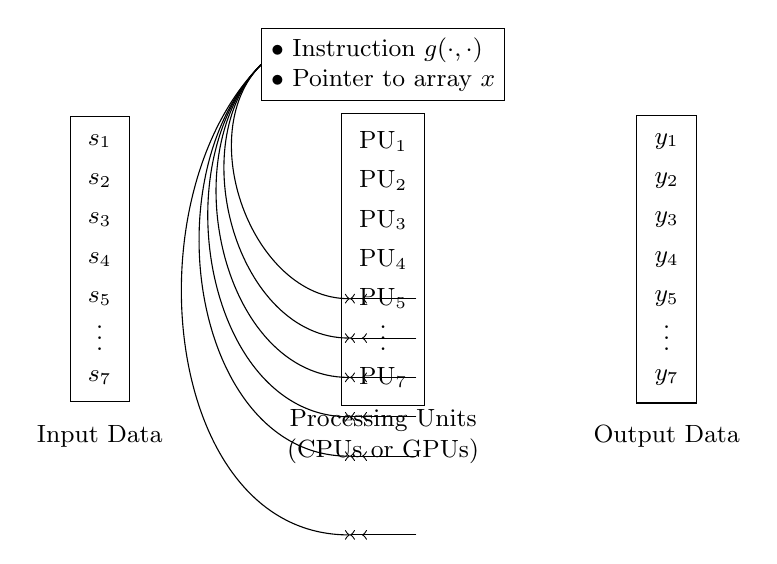
\begin{tikzpicture}[remember picture, scale=.9, font=\small]
    \node[draw,align=left] (I) at (0,2.75) {
      $\bullet$ Instruction $g(\cdot,\cdot)$\\
      $\bullet$ Pointer to array $x$
    };
    \node[draw] at (-4,0) {
      \tikz{
        \foreach\x in {1,2,3,4,5,7}{
          \node (A\x) at (0,-\x/2) {$s_{\x}$};
        }
        \node at (0,-2.9) {$\vdots$};
      }
    };
    \node[draw] at (0,0) {
      \tikz{
        \foreach\x in {1,2,3,4,5,7}{
          \node (B\x) at (0,-\x/2) {$\text{PU}_{\x}$};
        }
        \node at (0,-2.9) {$\vdots$};
      }
    };
    \node[draw] at (4,0) {
      \tikz{
        \foreach\x in {1,2,3,4,5,7}{
          \node (C\x) at (0,-\x/2) {$y_{\x}$};
        }
        \node at (0,-2.9) {$\vdots$};
      }
    };
    \foreach\x in {1,2,3,4,5,7}{
      \draw[->] (A\x.east) -- (B\x.west);
      \draw[->] (B\x.east) -- (C\x.west);
      \draw[->] (I.west) to [out=-135,in=180] (B\x.west);
    }
    \node at (-4,-2.5) {Input Data};
    \node[align=center] at (0,-2.5) {Processing Units\\(CPUs or GPUs)};
    \node at (4,-2.5) {Output Data};
  \end{tikzpicture}
  \label{fig:simd}
  \caption{A schematic description of SIMD parallelism}
\end{figure}


\section{SIMD Abstraction of Nonlinear Programs}\label{sec:simd}
\begin{subequations}\label{eqn:prob}
  \begin{align}
    \min_{x^L\leq x \leq x^U}& \sum_{\ell\in[L]}\sum_{i\in [I_k]} f^{(\ell)}(x; p^{(\ell)}_i)\\
    \st\; &\forall m\in[M]:\\
    &\begin{aligned}[t]
      g^{(m)}_\flat\leq &\left[g^{(m)}(x; q_j)\right]_{j\in [J]} \\
      &+\sum_{n\in [N_m]}\sum_{k\in [K_n]}h^{(n)}(x; s^{(n)}_{k}) \leq g^{(m)}_\sharp,
    \end{aligned}
  \end{align}
\end{subequations}
\section{Condensed-Space Interior Point Methods}\label{sec:ipm}

\section{Numerical Results}\label{sec:num}

\section{Conclusions and Future Outlook}\label{sec:conc}


\bibliographystyle{IEEEtran}
\bibliography{main}

\end{document}


